\documentclass[12pt,a4paper,oneside]{article}
\usepackage[utf8]{inputenc}
\usepackage{t1enc} % hyphenate accented chars
\usepackage[hungarian]{babel}
\usepackage{../fedlap}
\usepackage{fancyhdr} % elofej, elolab
\usepackage{graphicx}
\usepackage{datetime} % specify date format
\setcounter{secnumdepth}{3} % enable subsubsection

% hasonlitson a doc verziora
\addtolength{\voffset}{-1cm}

% cim
\csapat{nand}{39}
\konzulens{Bozóki Szilárd}
\datum{\todaynum}

% csapattagok
\taga{Berki Endre}{HQNHER}{berkiendre@gmail.com}
\tagb{Fodor Bertalan Ferenc}{H4T1UX}{foberci@gmail.com}
\tagc{Kádár András}{JFENWR}{arycika@gmail.com}
\tagd{Thaler Benedek}{EDDO10}{thalerbenedek@gmail.com}

\setlength{\headheight}{1.3em}
\setlength{\headsep}{2em}

% elofej, elolab
\fancyhf{}

\fancyhead[OL] { \tiny \leftmark{} }
\fancyhead[OR] { \tmpcsapat }

\fancyfoot[OR] { \thepage }
\fancyfoot[OL] { \tmpdatum }

\pagestyle{fancy}

% custom date format, according to customer request
% you have to use the \todaynum command instead of today,
% becouse babel overrides it, and I couldn't find a way to override
% it again. I was tempted to call this format \todaybozoki
\newcommand{\todaynum}{\the\year. \twodigit\month. \twodigit\day}


\begin{document}

\anyag{3. Analízis modell kidolgozása}
\fedlap

\addtocounter{section}{2}
\section{Analízis modell kidolgozása}

	\subsection{Objektum katalógus}
	
	\subsection{Osztályok leírása}
	
		\subsubsection{AbstractFrameItem}
		\begin{description}
		\item[Felelősség]
		Absztrakt ősosztály, a frameben lévő objektumokat testesíti meg (Platform, Door, Key, Stickman).
		\item[Ősosztályok] Object $\rightarrow{}$ AbstractFrameItem.
		\item[Interfészek] FrameItem.
		\item[Attribútumok]$\ $
		\begin{description}
		\item[] (nincs)
		\end{description}
		\item[Metódusok]$\ $
		\begin{description}
		\item[] (nincs)
		\end{description}
		\end{description}
		
		\subsubsection{Door}
		\begin{description}
		\item[Felelősség]
		A pályák befejezésére szolgáló ajtót valósítja meg.
		\item[Ősosztályok] Object $\rightarrow{}$ AbstractFrameItem $\rightarrow{}$ Door.
		\item[Interfészek] (nincs)
		\item[Attribútumok]$\ $
		\begin{description}
		\item[] (nincs)
		\end{description}
		\item[Metódusok]$\ $
		\begin{description}
		\item[] (nincs)
		\end{description}
		\end{description}
		
		\subsubsection{Frame}
		\begin{description}
		\item[Felelősség]
		Egy pályán belüli keret, amelyben mozoghat a stickman. Tartalmazza a pálya többi objektumát (Door, Key, Platform).
		\item[Ősosztályok] Object $\rightarrow{}$ Frame.
		\item[Interfészek] (nincs)
		\item[Attribútumok]$\ $
		\begin{description}
		\item[] (nincs)
		\end{description}
		\item[Metódusok]$\ $
		\begin{description}
		\item[] (nincs)
		\end{description}
		\end{description}
		
		\subsubsection{FrameItem}
		Interfész.
		\begin{description}
		\item[Felelősség]
		A Frame osztály ezen a felületen keresztül éri el a tartalmazott objektumokat.   Ezen interfacet valósítják meg a pályán lévő objektumok (Platform, Door, Key, Stickman)
		\item[Ősosztályok] FrameItem.
		\item[Interfészek] (nincs)
		\item[Metódusok]$\ $
		\begin{description}
		\item[] (nincs)
		\end{description}
		\end{description}
		
		\subsubsection{Game}
		\begin{description}
		\item[Felelősség]
		A játékot szervező objektum. Felelős az új pályák betöltéséért és a teljesített pályák törléséért.
		\item[Ősosztályok] Object $\rightarrow{}$ Game.
		\item[Interfészek] (nincs)
		\item[Attribútumok]$\ $
		\begin{description}
		\item[] (nincs)
		\end{description}
		\item[Metódusok]$\ $
		\begin{description}
		\item[] (nincs)
		\end{description}
		\end{description}
		
		\subsubsection{Key}
		\begin{description}
		\item[Felelősség]
		Kulcsok megszerzése a pálya teljesítésének feltétele.
		\item[Ősosztályok] Object $\rightarrow{}$ AbstractFrameItem $\rightarrow{}$ Key.
		\item[Interfészek] (nincs)
		\item[Attribútumok]$\ $
		\begin{description}
		\item[] (nincs)
		\end{description}
		\item[Metódusok]$\ $
		\begin{description}
			\item[\texttt{public boolean isCollected()}] \hfill \\
		 % TODO
		\end{description}
		\end{description}
		
		\subsubsection{Map}
		\begin{description}
		\item[Felelősség]
		Frameket tartalmazza, azokat mozgatja és kiválasztását irányítja.
		\item[Ősosztályok] Object $\rightarrow{}$ Map.
		\item[Interfészek] (nincs)
		\item[Attribútumok]$\ $
		\begin{description}
		\item[] (nincs)
		\end{description}
		\item[Metódusok]$\ $
		\begin{description}
		\item[] (nincs)
		\end{description}
		\end{description}
		
		\subsubsection{MapFactory}
		\begin{description}
		\item[Felelősség]
		Azonosító alapján Pályákat szolgáltat a Game objektum számára.
		\item[Ősosztályok] Object $\rightarrow{}$ MapFactory.
		\item[Interfészek] (nincs)
		\item[Attribútumok]$\ $
		\begin{description}
		\item[] (nincs)
		\end{description}
		\item[Metódusok]$\ $
		\begin{description}
		\item[] (nincs)
		\end{description}
		\end{description}
		
		\subsubsection{Platform}
		\begin{description}
		\item[Felelősség]
		A Stickman és ezzel a játék mozgásterét korlátozó objektum. A framen belül bejárható rész keretezése.
		\item[Ősosztályok] Object $\rightarrow{}$ AbstractFrameItem $\rightarrow{}$ Platform.
		\item[Interfészek] (nincs)
		\item[Attribútumok]$\ $
		\begin{description}
		\item[] (nincs)
		\end{description}
		\item[Metódusok]$\ $
		\begin{description}
		\item[] (nincs)
		\end{description}
		\end{description}
		
		\subsubsection{PubSub}
		\begin{description}
		\item[Felelősség]
		Globális üzenet közvetítő csatorna, mely a Publish/Subscribe mintát valósítja meg.
		\item[Ősosztályok] Object $\rightarrow{}$ PubSub.
		\item[Interfészek] (nincs)
		\item[Attribútumok]$\ $
		\begin{description}
		\item[] (nincs)
		\end{description}
		\item[Metódusok]$\ $
		\begin{description}
			\item[\texttt{public void emit(String eventName, Object data)}] \hfill \\Esemény történésének jelzése.
		\end{description}
		\end{description}
		
		\subsubsection{Stickman}
		\begin{description}
		\item[Felelősség]
		A játék által irányított figurát reprezentáló objektum.
		\item[Ősosztályok] Object $\rightarrow{}$ AbstractFrameItem $\rightarrow{}$ Stickman.
		\item[Interfészek] (nincs)
		\item[Attribútumok]$\ $
		\begin{description}
		\item[] (nincs)
		\end{description}
		\item[Metódusok]$\ $
		\begin{description}
		\item[] (nincs)
		\end{description}
		\end{description}
	
	\subsection{Szekvencia diagramok}
	
		\begin{figure}[h!]
			\begin{center}
				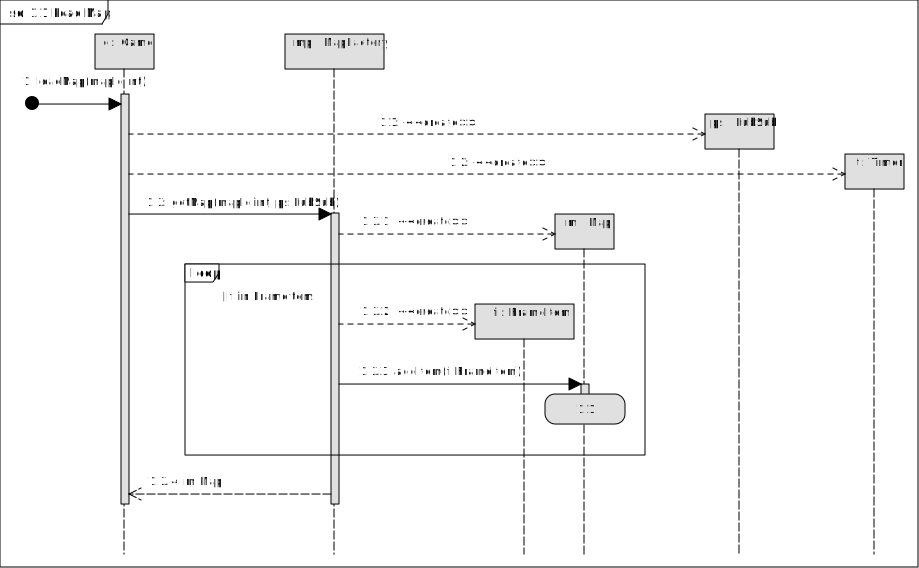
\includegraphics[scale=0.8]{resources/seq_1-0_newMap}
				% TODO caption
				\caption{}
			\end{center}
		\end{figure}
		
		\begin{figure}[h!]
			\begin{center}
				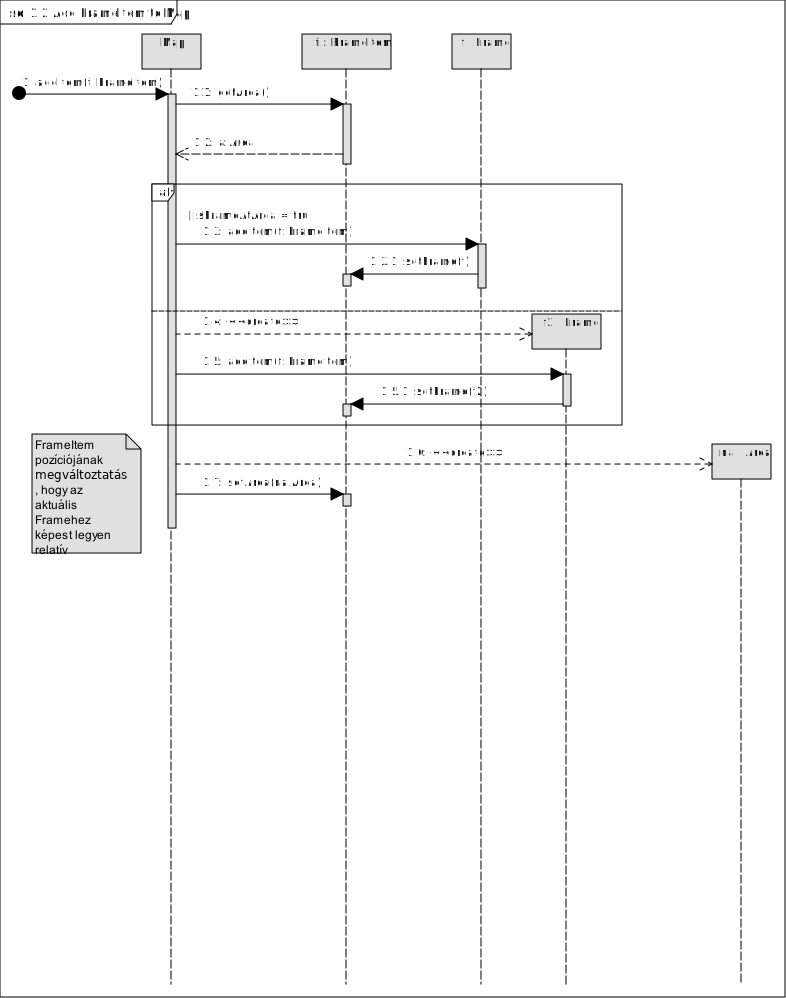
\includegraphics[scale=0.8]{resources/seq_1-1_addFrameItemToMap.png}
				% TODO
				\caption{}
			\end{center}
		\end{figure}
		
		\begin{figure}[h!]
			\begin{center}
				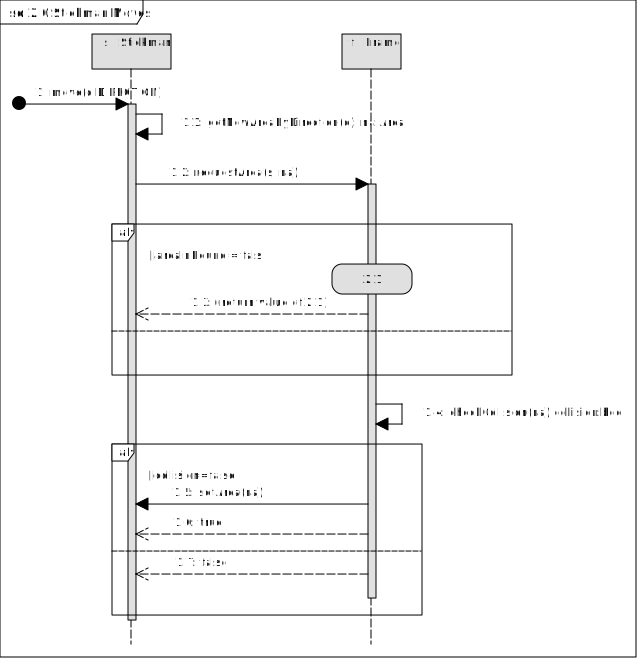
\includegraphics[scale=0.8]{resources/seq_2-0_stickmanMoves.png}
				% TODO
				\caption{}
			\end{center}
		\end{figure}
		
		\begin{figure}[h!]
			\begin{center}
				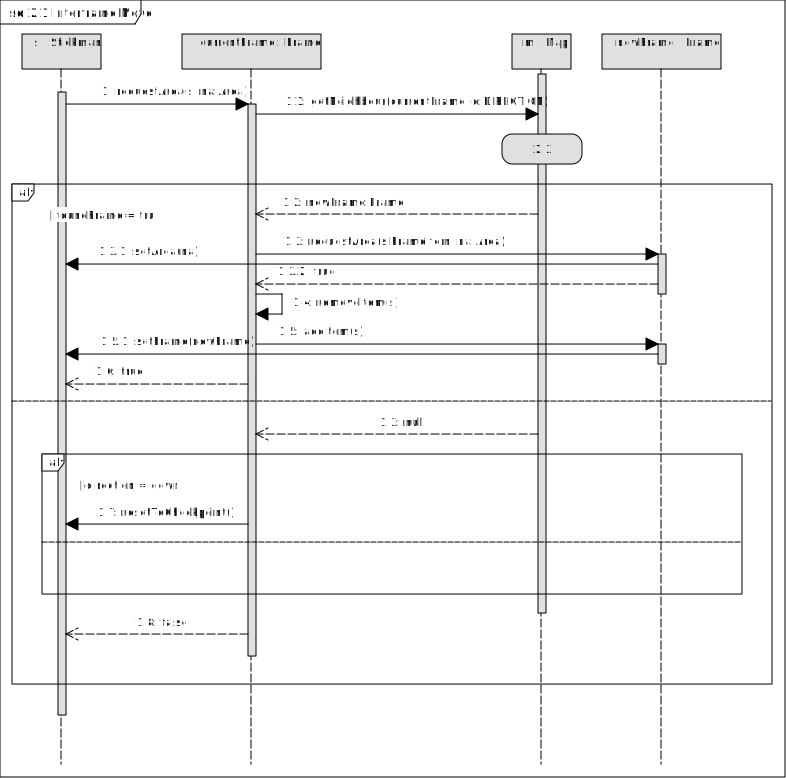
\includegraphics[scale=0.8]{resources/seq_2-1_interframeMove.png}
				% TODO
				\caption{}
			\end{center}
		\end{figure}
		
		\begin{figure}[h!]
			\begin{center}
				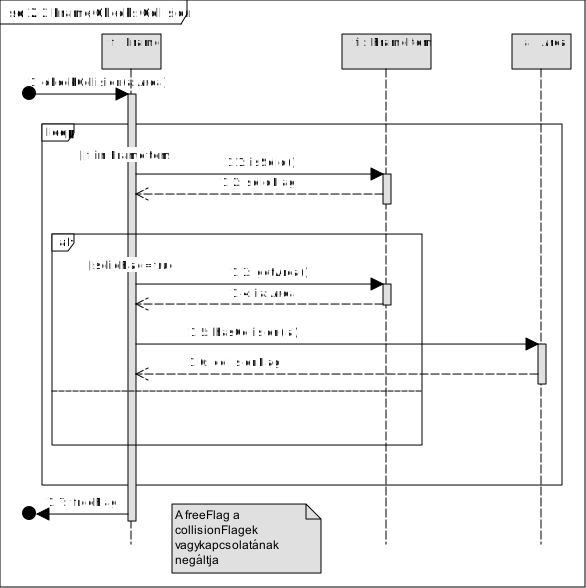
\includegraphics[scale=0.8]{resources/seq_2-2_frameChecksCollision.png}
				% TODO
				\caption{}
			\end{center}
		\end{figure}
		
		\begin{figure}[h!]
			\begin{center}
				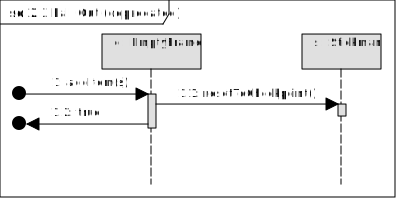
\includegraphics[scale=0.8]{resources/seq_2-3_fallOut.png}
				% TODO
				\caption{}
			\end{center}
		\end{figure}
		
		\begin{figure}[h!]
			\begin{center}
				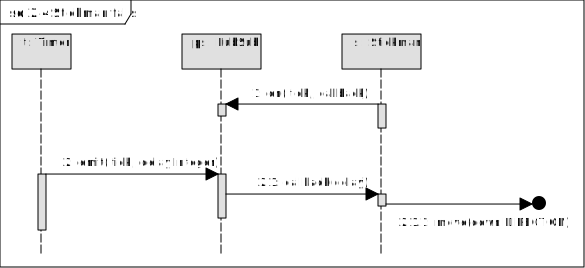
\includegraphics[scale=0.8]{resources/seq_2-4_stickmanFalls.png}
				% TODO
				\caption{}
			\end{center}
		\end{figure}
		
			\begin{figure}[h!]
			\begin{center}
			% TODO vegleges kep
				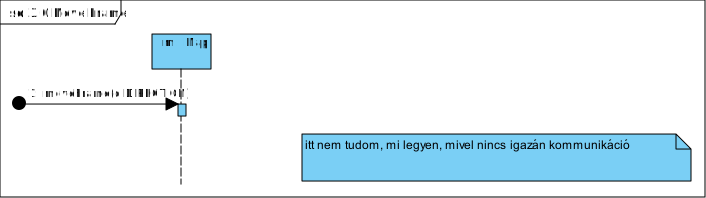
\includegraphics[scale=0.8]{resources/seq_3-0_moveFrame.png}
				% TODO
				\caption{}
			\end{center}
		\end{figure}
		
		
	
	\subsection{State-chartok}
	
	\begin{figure}[h!]
			\begin{center}
				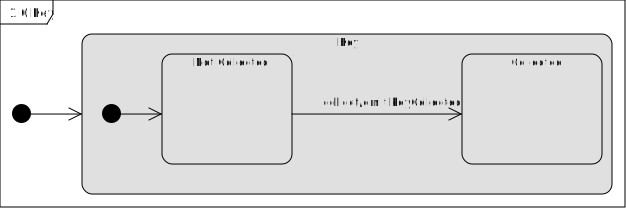
\includegraphics[scale=0.8]{resources/state_1-0_key.png}
				% TODO
				\caption{}
			\end{center}
		\end{figure}
		
		\begin{figure}[h!]
			\begin{center}
				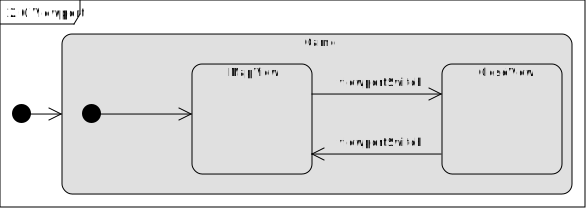
\includegraphics[scale=0.8]{resources/state_2-0_viewport.png}
				% TODO
				\caption{}
			\end{center}
		\end{figure}
	
	\subsection{Napló}
	% The diary generator uses the following comments to identify the beginning and the ending of the generated diary
	% The following content is auto generated, please do NOT modify, edit the related shared document instead.
	%GENERATOR:DIARY
	%GENERATOR:DIARY
\end{document}
